\documentclass[11pt]{article}
\usepackage{mathblatt}
% gesetzt von werkzeuge/setzer.py (Sorte selbst) aus dem Lernweg KUV
% und den Bankzeilen; Muster bau/proben/2026-10-09/hypotenuse-muster.
\usepackage{enumitem}
\newgeometry{a4paper,margin=18mm,top=15mm,bottom=20mm,footskip=9mm}
\pagestyle{fancy}\fancyhf{}\renewcommand{\headrulewidth}{0pt}
\fancyfoot[L]{\footnotesize\color{mbgrau}KUV \textperiodcentered{} Wahrscheinlichkeit: günstig durch möglich}
\fancyfoot[R]{\footnotesize\color{mbgrau}\thepage}
\setlength{\parskip}{3pt}
\renewcommand{\kreuz}[1]{\mbox{$\square$\ #1}\quad}
\newcommand{\kreuzl}[1]{\par\hangindent1.4em\hangafter1\noindent$\square$\ #1}
\newcommand{\aufg}[3]{\par\noindent\makebox[0pt][r]{#3}\begin{minipage}[t]{\linewidth}#1\end{minipage}\par}
\newcommand{\aufgg}[4]{\par\noindent\makebox[0pt][r]{#4}\begin{minipage}[t]{0.6\linewidth}\vspace{0pt}#1\end{minipage}\hfill
  \begin{minipage}[t]{0.37\linewidth}\vspace{0pt}\centering #2\end{minipage}\par}
\newcommand{\nr}[1]{\makebox[7mm][l]{\textbf{#1}}}
\newcommand{\lsg}[3]{\par\noindent\begin{minipage}[t]{9mm}\textbf{#1}\end{minipage}%
  \begin{minipage}[t]{52mm}\raggedright\bfseries\boldmath #2\end{minipage}\hspace{3mm}%
  \begin{minipage}[t]{\dimexpr\linewidth-64mm\relax}\raggedright\small #3\end{minipage}\par\vspace{4pt}}
\newlength{\kr}
\begin{document}

\noindent{\LARGE\bfseries Wahrscheinlichkeit: günstig durch möglich}\par\smallskip
\noindent{\small\color{mbgrau}Selbstlernheft Klasse 7 \textperiodcentered{} mit Lösungsheft \textperiodcentered{} Kennung KUV}\par\medskip
\noindent\textbf{So nutzt du das Heft:} Lies im Abschnitt das Beispiel. Rechne dann die Aufgaben der Reihe nach und vergleiche jede sofort mit dem Lösungsheft. Kreuze „kann ich“ an, wenn du die letzte Aufgabe (\emph{Ziel}) allein schaffst.\par
\noindent Mehr Aufgaben zu einem Abschnitt: Kennung deinem Nachhilfelehrer schicken (z.\,B. „KUV mehr B“).\par\medskip
{\arrayrulecolor{mbgrau}\renewcommand{\arraystretch}{1.3}
\noindent\begin{tabular}{|>{\bfseries}p{10mm}|p{112mm}|>{\raggedleft\arraybackslash}p{10mm}|>{\centering\arraybackslash}p{14mm}|}\hline
\rowcolor{black!8} & \textbf{Abschnitt} & \textbf{Seite} & \textbf{kann ich}\\\hline
A & Günstig durch möglich & \pageref{s:A} & $\square$\\\hline
B & Alle mitzählen, in Prozent & \pageref{s:B} & $\square$\\\hline
C & Gegenereignis: „nicht“ und „weder … noch“ & \pageref{s:C} & $\square$\\\hline
D & Wenn sich die Grundmenge ändert & \pageref{s:D} & $\square$\\\hline
E & Zufallsgerät bauen und vorhersagen & \pageref{s:E} & $\square$\\\hline
T & Probetest & \pageref{s:T} & $\square$\\\hline
\end{tabular}}\par\bigskip

\clearpage\label{s:A}\noindent\colorbox{black!12}{\makebox[10mm]{\Large\bfseries\strut A}}\hspace{3mm}{\Large\bfseries Günstig durch möglich}\par\smallskip
\noindent Sind alle Ergebnisse gleich wahrscheinlich (gleich große Felder, gleiche Kugeln, fairer Würfel), zählst du: Wie viele Ergebnisse sind \textbf{möglich}? Wie viele davon sind \textbf{günstig}, passen also zum Ereignis? Die Wahrscheinlichkeit ist günstig durch möglich.\par\medskip
\noindent\textbf{Formel}\par\nopagebreak\noindent\hspace*{4mm}\begin{minipage}{\dimexpr\linewidth-4mm\relax}$P(E) = \dfrac{\text{Anzahl der günstigen Ergebnisse}}{\text{Anzahl der möglichen Ergebnisse}}$ \qquad {\small Bruch kürzen.}\end{minipage}\par\medskip
\noindent\textbf{Beispiel}\quad Das Glücksrad hat 8 gleich große Felder mit den Zahlen 1 bis 8. Wie groß ist die Wahrscheinlichkeit für eine gerade Zahl?\par\smallskip
\noindent\begin{minipage}[t]{0.6\linewidth}\vspace{0pt}\par\noindent\hangindent6mm\hangafter1\makebox[6mm][l]{\textbf{1}}Möglich sind 8 Ergebnisse: 1, 2, \ldots, 8. Alle Felder sind gleich groß.\par\smallskip\par\noindent\hangindent6mm\hangafter1\makebox[6mm][l]{\textbf{2}}Günstig sind die geraden Zahlen 2, 4, 6, 8: das sind 4.\par\smallskip\par\noindent\hangindent6mm\hangafter1\makebox[6mm][l]{\textbf{3}}$P(\text{gerade}) = \dfrac{\text{günstig}}{\text{möglich}} = \dfrac{4}{8} = \dfrac{1}{2}$\par\smallskip\par\noindent\hangindent6mm\hangafter1\makebox[6mm][l]{\textbf{4}}Die Wahrscheinlichkeit für eine gerade Zahl ist $\frac{1}{2}$.\par\smallskip\end{minipage}\hfill
\begin{minipage}[t]{0.37\linewidth}\vspace{0pt}\centering 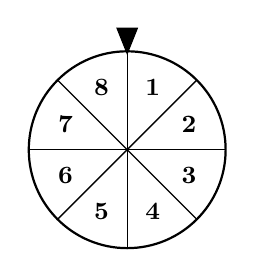
\begin{tikzpicture}[font=\small]\draw[line width=0.5pt] (0,0) -- (90.00:1.25);\node at (67.50:0.85) {\textbf{1}};\draw[line width=0.5pt] (0,0) -- (45.00:1.25);\node at (22.50:0.85) {\textbf{2}};\draw[line width=0.5pt] (0,0) -- (0.00:1.25);\node at (-22.50:0.85) {\textbf{3}};\draw[line width=0.5pt] (0,0) -- (-45.00:1.25);\node at (-67.50:0.85) {\textbf{4}};\draw[line width=0.5pt] (0,0) -- (-90.00:1.25);\node at (-112.50:0.85) {\textbf{5}};\draw[line width=0.5pt] (0,0) -- (-135.00:1.25);\node at (-157.50:0.85) {\textbf{6}};\draw[line width=0.5pt] (0,0) -- (-180.00:1.25);\node at (-202.50:0.85) {\textbf{7}};\draw[line width=0.5pt] (0,0) -- (-225.00:1.25);\node at (-247.50:0.85) {\textbf{8}};\draw[line width=0.8pt] (0,0) circle (1.25);\fill (0,1.20) -- (-0.14,1.55) -- (0.14,1.55) -- cycle;\end{tikzpicture}\end{minipage}\par\medskip
\noindent\textbf{Aufgaben}\hspace{1em}{\small\color{mbgrau}Rechne unten im Karo. Vergleiche jede Aufgabe gleich mit dem Lösungsheft.}\par\smallskip
\aufg{\hangindent7mm\hangafter1\nr{1.}Ein Würfel wird einmal geworfen. Wie groß ist die Wahrscheinlichkeit für eine 5?}{}{}
\medskip
\aufg{\hangindent7mm\hangafter1\nr{2.}In einem Beutel liegen 4 rote, 7 blaue und 1 weiße Kugel. Lisa zieht ohne hinzusehen eine Kugel. Wie groß ist die Wahrscheinlichkeit für Blau?}{}{}
\medskip
\aufgg{\hangindent7mm\hangafter1\nr{3.}Das Glücksrad im Bild hat 6 gleich große Felder. Wie groß ist die Wahrscheinlichkeit für A?}{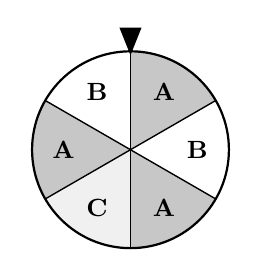
\begin{tikzpicture}[font=\small]\fill[black!22] (0,0) -- (90.00:1.25) arc (90.00:30.00:1.25) -- cycle;\draw[line width=0.5pt] (0,0) -- (90.00:1.25);\node at (60.00:0.85) {\textbf{A}};\draw[line width=0.5pt] (0,0) -- (30.00:1.25);\node at (0.00:0.85) {\textbf{B}};\fill[black!22] (0,0) -- (-30.00:1.25) arc (-30.00:-90.00:1.25) -- cycle;\draw[line width=0.5pt] (0,0) -- (-30.00:1.25);\node at (-60.00:0.85) {\textbf{A}};\fill[black!6] (0,0) -- (-90.00:1.25) arc (-90.00:-150.00:1.25) -- cycle;\draw[line width=0.5pt] (0,0) -- (-90.00:1.25);\node at (-120.00:0.85) {\textbf{C}};\fill[black!22] (0,0) -- (-150.00:1.25) arc (-150.00:-210.00:1.25) -- cycle;\draw[line width=0.5pt] (0,0) -- (-150.00:1.25);\node at (-180.00:0.85) {\textbf{A}};\draw[line width=0.5pt] (0,0) -- (-210.00:1.25);\node at (-240.00:0.85) {\textbf{B}};\draw[line width=0.8pt] (0,0) circle (1.25);\fill (0,1.20) -- (-0.14,1.55) -- (0.14,1.55) -- cycle;\end{tikzpicture}}{}{}
\medskip
\aufg{\hangindent7mm\hangafter1\nr{4.}In einer Schachtel liegen 20 Zettel mit den Zahlen 1 bis 20. Tom zieht einen Zettel. Wie groß ist die Wahrscheinlichkeit, dass die Zahl durch 5 teilbar ist?}{}{}
\medskip
\aufg{\hangindent7mm\hangafter1\nr{5.}Lena darf aus einem von zwei Beuteln eine Kugel ziehen. Bei Rot gewinnt sie. Im ersten Beutel sind 3 rote und 5 grüne Kugeln, im zweiten 4 rote und 8 grüne. Aus welchem Beutel sollte sie ziehen? Begründe mit den Wahrscheinlichkeiten.}{}{{\scriptsize\color{mbgrau}Ziel\hspace{2mm}}}
\medskip
\par\vspace{3mm}\setlength{\kr}{\dimexpr\pagegoal-\pagetotal-10mm\relax}%
\ifdim\kr>12mm\noindent{\scriptsize\color{mbgrau}Platz zum Rechnen}\par\nointerlineskip\vspace{1mm}\noindent
\begin{tikzpicture}\clip (0,0) rectangle ({\linewidth-0.5mm},\kr);\draw[black!16,line width=0.3pt,step=5mm] (0,0) grid (\linewidth,\kr);\end{tikzpicture}\fi\par
\clearpage\label{s:B}\noindent\colorbox{black!12}{\makebox[10mm]{\Large\bfseries\strut B}}\hspace{3mm}{\Large\bfseries Alle mitzählen, in Prozent}\par\smallskip
\noindent Lies genau, was alles in der Trommel, der Kiste oder dem Beutel liegt: Möglich sind \emph{alle} Stücke, auch Nieten und kaputte. Für die Prozentangabe teilst du Zähler durch Nenner und nimmst mal 100.\par\medskip
\noindent\textbf{Formel}\par\nopagebreak\noindent\hspace*{4mm}\begin{minipage}{\dimexpr\linewidth-4mm\relax}alle $=$ günstige $+$ übrige \qquad $\frac{1}{4} = 1 : 4 = 0{,}25 = 25\,\%$\end{minipage}\par\medskip
\noindent\textbf{Beispiel}\quad In einer Lostrommel liegen 36 Nieten und 12 Gewinne. Wie groß ist die Wahrscheinlichkeit für einen Gewinn? Gib sie als Bruch, als Dezimalzahl und in Prozent an.\par\smallskip
\noindent\par\noindent\hangindent6mm\hangafter1\makebox[6mm][l]{\textbf{1}}Möglich sind alle Lose: $36 + 12 = 48$. Die Nieten zählen mit!\par\smallskip\par\noindent\hangindent6mm\hangafter1\makebox[6mm][l]{\textbf{2}}Günstig sind die 12 Gewinne.\par\smallskip\par\noindent\hangindent6mm\hangafter1\makebox[6mm][l]{\textbf{3}}$P = \dfrac{12}{48} = \dfrac{1}{4}$\par\smallskip\par\noindent\hangindent6mm\hangafter1\makebox[6mm][l]{\textbf{4}}Dezimalzahl: $1 : 4 = 0{,}25$. Prozent: $0{,}25 = 25\,\%$.\par\smallskip\par\noindent\hangindent6mm\hangafter1\makebox[6mm][l]{\textbf{5}}\textbf{Zählen mit Nummern:} Tragen die Lose die Nummern 11 bis 58, sind es $58 - 11 + 1 = 48$ Lose – plus 1, weil die erste Nummer mitzählt.\par\smallskip\par\medskip
\noindent\textbf{Aufgaben}\hspace{1em}{\small\color{mbgrau}Rechne unten im Karo. Vergleiche jede Aufgabe gleich mit dem Lösungsheft.}\par\smallskip
\aufg{\hangindent7mm\hangafter1\nr{1.}Die Wahrscheinlichkeit für Rot ist $\frac{3}{5}$. Schreibe sie als Dezimalzahl und in Prozent.}{}{}
\medskip
\aufg{\hangindent7mm\hangafter1\nr{2.}In einer Kiste liegen 54 volle und 6 leere Batterien. Jan nimmt ohne hinzusehen eine heraus. Wie groß ist die Wahrscheinlichkeit, dass sie leer ist? Gib sie in Prozent an.}{}{}
\medskip
\aufg{\hangindent7mm\hangafter1\nr{3.}In einer Tüte sind 11 rote, 6 grüne und 8 gelbe Gummibärchen. Wie groß ist die Wahrscheinlichkeit, ein rotes zu ziehen? Gib sie in Prozent an.}{}{}
\medskip
\aufg{\hangindent7mm\hangafter1\nr{4.}Die Lose einer Tombola tragen die Nummern 201 bis 600. Die Lose mit den Nummern 201 bis 250 gewinnen. Wie groß ist die Wahrscheinlichkeit für einen Gewinn? Gib sie in Prozent an.}{}{}
\medskip
\aufg{\hangindent7mm\hangafter1\nr{5.}Beim Schulfest gibt es zwei Losbuden. In Bude A sind 150 Nieten und 50 Gewinne. In Bude B sind 300 Lose, davon 66 Gewinne. Max will ein Los dort kaufen, wo seine Chance besser ist. Welche Bude wählt er? Gib beide Chancen in Prozent an.}{}{{\scriptsize\color{mbgrau}Ziel\hspace{2mm}}}
\medskip
\par\vspace{3mm}\setlength{\kr}{\dimexpr\pagegoal-\pagetotal-10mm\relax}%
\ifdim\kr>12mm\noindent{\scriptsize\color{mbgrau}Platz zum Rechnen}\par\nointerlineskip\vspace{1mm}\noindent
\begin{tikzpicture}\clip (0,0) rectangle ({\linewidth-0.5mm},\kr);\draw[black!16,line width=0.3pt,step=5mm] (0,0) grid (\linewidth,\kr);\end{tikzpicture}\fi\par
\clearpage\label{s:C}\noindent\colorbox{black!12}{\makebox[10mm]{\Large\bfseries\strut C}}\hspace{3mm}{\Large\bfseries Gegenereignis: „nicht“ und „weder … noch“}\par\smallskip
\noindent Das \textbf{Gegenereignis} ist alles, was nicht zum Ereignis gehört. Beide zusammen haben die Wahrscheinlichkeit 1 (100\,\%). Oft ist das Gegenteil leichter zu zählen.\par\medskip
\noindent\textbf{Formel}\par\nopagebreak\noindent\hspace*{4mm}\begin{minipage}{\dimexpr\linewidth-4mm\relax}$P(\text{nicht } E) = 1 - P(E)$ \qquad in Prozent: $100\,\% - P(E)$\end{minipage}\par\medskip
\noindent\textbf{Beispiel}\quad Ein Glücksrad hat 10 gleich große Felder mit den Zahlen 1 bis 10. Wie groß ist die Wahrscheinlichkeit, weder die 1 noch die 10 zu drehen?\par\smallskip
\noindent\begin{minipage}[t]{0.6\linewidth}\vspace{0pt}\par\noindent\hangindent6mm\hangafter1\makebox[6mm][l]{\textbf{1}}Das Gegenteil von „weder 1 noch 10“ ist „1 oder 10“: 2 von 10 Feldern.\par\smallskip\par\noindent\hangindent6mm\hangafter1\makebox[6mm][l]{\textbf{2}}$P(1 \text{ oder } 10) = \dfrac{2}{10}$\par\smallskip\par\noindent\hangindent6mm\hangafter1\makebox[6mm][l]{\textbf{3}}$P(\text{weder 1 noch 10}) = 1 - \dfrac{2}{10} = \dfrac{8}{10} = \dfrac{4}{5}$\par\smallskip\par\noindent\hangindent6mm\hangafter1\makebox[6mm][l]{\textbf{4}}Probe durch Zählen: 2, 3, \ldots, 9 sind 8 Felder, also $\frac{8}{10}$.\par\smallskip\end{minipage}\hfill
\begin{minipage}[t]{0.37\linewidth}\vspace{0pt}\centering 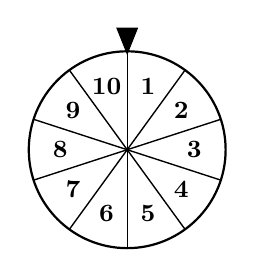
\begin{tikzpicture}[font=\small]\draw[line width=0.5pt] (0,0) -- (90.00:1.25);\node at (72.00:0.85) {\textbf{1}};\draw[line width=0.5pt] (0,0) -- (54.00:1.25);\node at (36.00:0.85) {\textbf{2}};\draw[line width=0.5pt] (0,0) -- (18.00:1.25);\node at (0.00:0.85) {\textbf{3}};\draw[line width=0.5pt] (0,0) -- (-18.00:1.25);\node at (-36.00:0.85) {\textbf{4}};\draw[line width=0.5pt] (0,0) -- (-54.00:1.25);\node at (-72.00:0.85) {\textbf{5}};\draw[line width=0.5pt] (0,0) -- (-90.00:1.25);\node at (-108.00:0.85) {\textbf{6}};\draw[line width=0.5pt] (0,0) -- (-126.00:1.25);\node at (-144.00:0.85) {\textbf{7}};\draw[line width=0.5pt] (0,0) -- (-162.00:1.25);\node at (-180.00:0.85) {\textbf{8}};\draw[line width=0.5pt] (0,0) -- (-198.00:1.25);\node at (-216.00:0.85) {\textbf{9}};\draw[line width=0.5pt] (0,0) -- (-234.00:1.25);\node at (-252.00:0.85) {\textbf{10}};\draw[line width=0.8pt] (0,0) circle (1.25);\fill (0,1.20) -- (-0.14,1.55) -- (0.14,1.55) -- cycle;\end{tikzpicture}\end{minipage}\par\medskip
\noindent\textbf{Aufgaben}\hspace{1em}{\small\color{mbgrau}Rechne unten im Karo. Vergleiche jede Aufgabe gleich mit dem Lösungsheft.}\par\smallskip
\aufg{\hangindent7mm\hangafter1\nr{1.}Die Wahrscheinlichkeit, bei einem Spiel zu gewinnen, ist 0,3. Wie groß ist die Wahrscheinlichkeit, nicht zu gewinnen?}{}{}
\medskip
\aufg{\hangindent7mm\hangafter1\nr{2.}Ein Würfel wird einmal geworfen. Wie groß ist die Wahrscheinlichkeit, keine 6 zu würfeln?}{}{}
\medskip
\aufg{\hangindent7mm\hangafter1\nr{3.}In einem Beutel liegen 5 rote, 3 blaue und 4 grüne Kugeln. Wie groß ist die Wahrscheinlichkeit, keine grüne Kugel zu ziehen?}{}{}
\medskip
\aufg{\hangindent7mm\hangafter1\nr{4.}Ein Glücksrad hat 12 gleich große Felder mit den Zahlen 1 bis 12. Wie groß ist die Wahrscheinlichkeit für eine Zahl, die weder durch 3 noch durch 4 teilbar ist?}{}{}
\medskip
\aufg{\hangindent7mm\hangafter1\nr{5.}Ole und Mia spielen mit einem Würfel. Ole gewinnt, wenn weder eine 1 noch eine 2 fällt. Sonst gewinnt Mia. Ole sagt: „Das Spiel ist fair. Wir haben die gleiche Chance.“ Hat Ole recht?}{}{{\scriptsize\color{mbgrau}Ziel\hspace{2mm}}}
\medskip
\par\vspace{3mm}\setlength{\kr}{\dimexpr\pagegoal-\pagetotal-10mm\relax}%
\ifdim\kr>12mm\noindent{\scriptsize\color{mbgrau}Platz zum Rechnen}\par\nointerlineskip\vspace{1mm}\noindent
\begin{tikzpicture}\clip (0,0) rectangle ({\linewidth-0.5mm},\kr);\draw[black!16,line width=0.3pt,step=5mm] (0,0) grid (\linewidth,\kr);\end{tikzpicture}\fi\par
\clearpage\label{s:D}\noindent\colorbox{black!12}{\makebox[10mm]{\Large\bfseries\strut D}}\hspace{3mm}{\Large\bfseries Wenn sich die Grundmenge ändert}\par\smallskip
\noindent Ist schon etwas weg (gegessen, gezogen und nicht zurückgelegt), gibt es weniger mögliche Ergebnisse. Weißt du schon etwas (z.\,B. die letzte Ziffer), zählst du nur noch die Ergebnisse, die dazu passen.\par\medskip
\noindent\textbf{Formel}\par\nopagebreak\noindent\hspace*{4mm}\begin{minipage}{\dimexpr\linewidth-4mm\relax}$P = \dfrac{\text{günstige, die noch in Frage kommen}}{\text{alle, die noch in Frage kommen}}$\end{minipage}\par\medskip
\noindent\textbf{Beispiel}\quad In einer Dose liegen 20 Kekse, 4 davon mit Nuss. Nina hat schon 2 Kekse ohne Nuss gegessen. Wie groß ist jetzt die Wahrscheinlichkeit, einen Nusskeks zu erwischen?\par\smallskip
\noindent\par\noindent\hangindent6mm\hangafter1\makebox[6mm][l]{\textbf{1}}Noch in der Dose: $20 - 2 = 18$ Kekse.\par\smallskip\par\noindent\hangindent6mm\hangafter1\makebox[6mm][l]{\textbf{2}}Die Nusskekse sind noch alle da: 4.\par\smallskip\par\noindent\hangindent6mm\hangafter1\makebox[6mm][l]{\textbf{3}}$P(\text{Nuss}) = \dfrac{4}{18} = \dfrac{2}{9}$ – nicht $\dfrac{4}{20}$.\par\smallskip\par\medskip
\noindent\textbf{Aufgaben}\hspace{1em}{\small\color{mbgrau}Rechne unten im Karo. Vergleiche jede Aufgabe gleich mit dem Lösungsheft.}\par\smallskip
\aufg{\hangindent7mm\hangafter1\nr{1.}In einem Beutel sind 3 rote und 7 blaue Kugeln. Tim zieht eine blaue Kugel und legt sie nicht zurück. Wie groß ist jetzt die Wahrscheinlichkeit für Rot?}{}{}
\medskip
\aufg{\hangindent7mm\hangafter1\nr{2.}In einem Beutel sind 5 gelbe und 7 grüne Kugeln. Ela zieht eine gelbe Kugel und legt sie nicht zurück. Wie groß ist jetzt die Wahrscheinlichkeit, wieder Gelb zu ziehen?}{}{}
\medskip
\aufg{\hangindent7mm\hangafter1\nr{3.}Lose tragen die Nummern 101 bis 350. Einen Preis bekommt jedes Los, dessen Nummer auf 13 endet. Mia sieht von ihrem Los nur die letzte Ziffer: eine 3. Wie groß ist die Wahrscheinlichkeit, dass sie einen Preis bekommt? Gib sie auch in Prozent an.}{}{}
\medskip
\aufg{\hangindent7mm\hangafter1\nr{4.}Beim Sommerfest gibt es Lose mit den Nummern 301 bis 800. Einen Trostpreis bekommt jedes Los, dessen Nummer auf 27 endet – außer dem Los 527, das ist der Hauptgewinn. Jonas sieht von seinem Los nur die letzte Ziffer: eine 7. Er sagt: „Meine Chance auf einen Trostpreis ist größer als 10\,\%.“ Hat Jonas recht?}{}{{\scriptsize\color{mbgrau}Ziel\hspace{2mm}}}
\medskip
\par\vspace{3mm}\setlength{\kr}{\dimexpr\pagegoal-\pagetotal-10mm\relax}%
\ifdim\kr>12mm\noindent{\scriptsize\color{mbgrau}Platz zum Rechnen}\par\nointerlineskip\vspace{1mm}\noindent
\begin{tikzpicture}\clip (0,0) rectangle ({\linewidth-0.5mm},\kr);\draw[black!16,line width=0.3pt,step=5mm] (0,0) grid (\linewidth,\kr);\end{tikzpicture}\fi\par
\clearpage\label{s:E}\noindent\colorbox{black!12}{\makebox[10mm]{\Large\bfseries\strut E}}\hspace{3mm}{\Large\bfseries Zufallsgerät bauen und vorhersagen}\par\smallskip
\noindent Ist die Wahrscheinlichkeit gegeben, rechnest du rückwärts: So viele Felder oder Kugeln brauchst du. Genauso sagst du voraus, wie oft etwas bei vielen Versuchen \emph{ungefähr} eintritt – sicher ist das nicht.\par\medskip
\noindent\textbf{Formel}\par\nopagebreak\noindent\hspace*{4mm}\begin{minipage}{\dimexpr\linewidth-4mm\relax}günstige Felder $= P \cdot$ alle Felder \qquad erwartete Anzahl $= P \cdot$ Anzahl der Versuche\end{minipage}\par\medskip
\noindent\textbf{Beispiel}\quad Ein Glücksrad soll 10 gleich große Felder bekommen. Die Wahrscheinlichkeit für Gelb soll 30\,\% sein. a) Wie viele Felder färbst du gelb? b) Das Rad wird 200-mal gedreht. Wie oft kommt ungefähr Gelb?\par\smallskip
\noindent\par\noindent\hangindent6mm\hangafter1\makebox[6mm][l]{\textbf{1}}$30\,\% = 0{,}3$\par\smallskip\par\noindent\hangindent6mm\hangafter1\makebox[6mm][l]{\textbf{2}}a) gelbe Felder: $0{,}3 \cdot 10 = 3$\par\smallskip\par\noindent\hangindent6mm\hangafter1\makebox[6mm][l]{\textbf{3}}b) erwartet: $0{,}3 \cdot 200 = 60$-mal\par\smallskip\par\noindent\hangindent6mm\hangafter1\makebox[6mm][l]{\textbf{4}}„Ungefähr“: Es können auch 55 oder 64 sein. Die Wahrscheinlichkeit sagt nicht genau voraus.\par\smallskip\par\medskip
\noindent\textbf{Aufgaben}\hspace{1em}{\small\color{mbgrau}Rechne unten im Karo. Vergleiche jede Aufgabe gleich mit dem Lösungsheft.}\par\smallskip
\aufg{\hangindent7mm\hangafter1\nr{1.}Ein Glücksrad hat 8 gleich große Felder. Die Wahrscheinlichkeit für Rot soll $\frac{1}{4}$ sein. Wie viele Felder müssen rot sein?}{}{}
\medskip
\aufg{\hangindent7mm\hangafter1\nr{2.}In einem Beutel liegen 4 schwarze Kugeln. Wie viele weiße Kugeln musst du dazulegen, damit die Wahrscheinlichkeit für Schwarz $\frac{1}{3}$ ist?}{}{}
\medskip
\aufg{\hangindent7mm\hangafter1\nr{3.}Lukas würfelt 300-mal. Die 6 fällt 52-mal. Berechne die relative Häufigkeit der 6 (relative Häufigkeit = Treffer : Versuche) und vergleiche sie mit der Wahrscheinlichkeit für eine 6.}{}{}
\medskip
\aufg{\hangindent7mm\hangafter1\nr{4.}Auf dem Kinderfest dreht jedes Kind einmal ein Glücksrad mit 16 gleich großen Feldern. Auf 2 Feldern gewinnt man einen Teddy. Erwartet werden 480 Kinder. Es gibt 50 Teddys. Reichen sie?}{}{{\scriptsize\color{mbgrau}Ziel\hspace{2mm}}}
\medskip
\par\vspace{3mm}\setlength{\kr}{\dimexpr\pagegoal-\pagetotal-10mm\relax}%
\ifdim\kr>12mm\noindent{\scriptsize\color{mbgrau}Platz zum Rechnen}\par\nointerlineskip\vspace{1mm}\noindent
\begin{tikzpicture}\clip (0,0) rectangle ({\linewidth-0.5mm},\kr);\draw[black!16,line width=0.3pt,step=5mm] (0,0) grid (\linewidth,\kr);\end{tikzpicture}\fi\par
\clearpage\label{s:T}\noindent\colorbox{black!12}{\makebox[10mm]{\Large\bfseries\strut T}}\hspace{3mm}{\Large\bfseries Probetest}\par\smallskip
\noindent Gemischt wie in der Prüfung, ohne Beispiel. Taschenrechner erlaubt. Etwa 20 Minuten.\par\medskip\noindent\textbf{Typische Fehler – so nicht}\par\smallskip\noindent\nr{$\times$}Nieten nicht mitgezählt: $\frac{12}{36}$ statt $\frac{12}{48}$. Alle Lose sind möglich.\par\noindent\nr{$\times$}Farben gezählt statt Felder: $\frac{1}{3}$ bei drei Farben. Zähl die Felder.\par\noindent\nr{$\times$}Mehr rote Kugeln heißt nicht bessere Chance. Es zählt der Anteil.\par\noindent\nr{$\times$}Etwas ist schon weg, aber die alte Gesamtzahl genommen.\par\noindent\nr{$\times$}„Etwa 60-mal“ als „genau 60-mal“ gelesen.\par\par\medskip
\noindent\textbf{Aufgaben}\hspace{1em}{\small\color{mbgrau}Rechne unten im Karo. Vergleiche jede Aufgabe gleich mit dem Lösungsheft.}\par\smallskip
\aufgg{\hangindent7mm\hangafter1\nr{1.}Das Glücksrad im Bild hat 8 gleich große Felder (R rot, B blau, G grün). Wie groß ist die Wahrscheinlichkeit für Rot? Kreuze an.\par\smallskip\leftskip7mm \kreuz{$\frac{1}{3}$}\ \kreuz{$\frac{1}{2}$}\par\kreuz{$\frac{3}{8}$}\ \kreuz{$\frac{1}{4}$}}{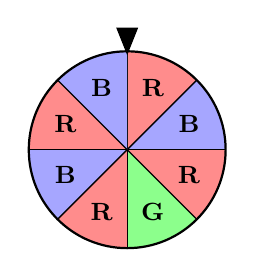
\begin{tikzpicture}[font=\small]\fill[red!45] (0,0) -- (90.00:1.25) arc (90.00:45.00:1.25) -- cycle;\draw[line width=0.5pt] (0,0) -- (90.00:1.25);\node at (67.50:0.85) {\textbf{R}};\fill[blue!35] (0,0) -- (45.00:1.25) arc (45.00:0.00:1.25) -- cycle;\draw[line width=0.5pt] (0,0) -- (45.00:1.25);\node at (22.50:0.85) {\textbf{B}};\fill[red!45] (0,0) -- (0.00:1.25) arc (0.00:-45.00:1.25) -- cycle;\draw[line width=0.5pt] (0,0) -- (0.00:1.25);\node at (-22.50:0.85) {\textbf{R}};\fill[green!45] (0,0) -- (-45.00:1.25) arc (-45.00:-90.00:1.25) -- cycle;\draw[line width=0.5pt] (0,0) -- (-45.00:1.25);\node at (-67.50:0.85) {\textbf{G}};\fill[red!45] (0,0) -- (-90.00:1.25) arc (-90.00:-135.00:1.25) -- cycle;\draw[line width=0.5pt] (0,0) -- (-90.00:1.25);\node at (-112.50:0.85) {\textbf{R}};\fill[blue!35] (0,0) -- (-135.00:1.25) arc (-135.00:-180.00:1.25) -- cycle;\draw[line width=0.5pt] (0,0) -- (-135.00:1.25);\node at (-157.50:0.85) {\textbf{B}};\fill[red!45] (0,0) -- (-180.00:1.25) arc (-180.00:-225.00:1.25) -- cycle;\draw[line width=0.5pt] (0,0) -- (-180.00:1.25);\node at (-202.50:0.85) {\textbf{R}};\fill[blue!35] (0,0) -- (-225.00:1.25) arc (-225.00:-270.00:1.25) -- cycle;\draw[line width=0.5pt] (0,0) -- (-225.00:1.25);\node at (-247.50:0.85) {\textbf{B}};\draw[line width=0.8pt] (0,0) circle (1.25);\fill (0,1.20) -- (-0.14,1.55) -- (0.14,1.55) -- cycle;\end{tikzpicture}}{}{}
\medskip
\aufg{\hangindent7mm\hangafter1\nr{2.}In einer Lostrommel liegen 104 Nieten und 16 Gewinne. Wie groß ist die Wahrscheinlichkeit für einen Gewinn? Gib sie in Prozent an.}{}{}
\medskip
\aufg{\hangindent7mm\hangafter1\nr{3.}Ein Glücksrad hat 12 gleich große Felder mit den Zahlen 1 bis 12. Wie groß ist die Wahrscheinlichkeit, keine Zahl über 9 zu drehen?}{}{}
\medskip
\aufg{\hangindent7mm\hangafter1\nr{4.}In einer Schale liegen 15 Bonbons, 3 davon mit Zitrone, die anderen mit Kirsche. Tom isst 3 Kirschbonbons. Sara sagt: „Die Wahrscheinlichkeit für Zitrone ist immer noch $\frac{3}{15}$.“ Hat Sara recht? Begründe.}{}{}
\medskip
\aufg{\hangindent7mm\hangafter1\nr{5.}Eine Klasse baut für das Schulfest ein Glücksrad mit 12 gleich großen Feldern. Ein Preis soll mit der Wahrscheinlichkeit 25\,\% kommen. Erwartet werden 300 Drehungen. Die Klasse hat 70 Preise. Wie viele Felder werden Preisfelder? Reichen die Preise?}{}{{\scriptsize\color{mbgrau}Ziel\hspace{2mm}}}
\medskip
\par\vspace{3mm}\setlength{\kr}{\dimexpr\pagegoal-\pagetotal-10mm\relax}%
\ifdim\kr>12mm\noindent{\scriptsize\color{mbgrau}Platz zum Rechnen}\par\nointerlineskip\vspace{1mm}\noindent
\begin{tikzpicture}\clip (0,0) rectangle ({\linewidth-0.5mm},\kr);\draw[black!16,line width=0.3pt,step=5mm] (0,0) grid (\linewidth,\kr);\end{tikzpicture}\fi\par
\end{document}
